%%%%%%%%%%%%%%%%%%%%%%%%%%%%%%%%%%%%%%%%%%%%%%%%%%%%%%%%%%%%%%%%%%%%%%%%%%%%%%%%%%%%%%%%%%%%%%%%%%%%%%%%%%%%%%%%%
%                               LaTeX TEMPLATE FOR ECOC 2022
%
%%%%%%%%%%%%%%%%%%%%%%%%%%%%%%%%%%%%%%%%%%%%%%%%%%%%%%%%%%%%%%%%%%%%%%%%%%%%%%%%%%%%%%%%%%%%%%%%%%%%%%%%%%%%%%%%%

%%%%%%%%%%%%%%%%%%%%%%%%%%%%%%%%%%%%%%%%%%%%%%%%%%%%%%%%%%%%%%%%%%%%%%%%%%%%%%%%%%%%%%%%%%%%%%%%%%%%%%%%%%%%%%%%%
% NOTES FOR USE:
%
% This template is meant to be used with PDF-LaTeX
%
%%%%%%%%%%%%%%%%%%%%%%%%%%%%%%%%%%%%%%%%%%%%%%%%%%%%%%%%%%%%%%%%%%%%%%%%%%%%%%%%%%%%%%%%%%%%%%%%%%%%%%%%%%%%%%%%%

%---------------------------------------------- Documentclass --------------------------------------------------%

\documentclass[a4paper, oneside, twocolumn, notitlepage, 10pt]{extarticle_ecoc}
\usepackage{ecoc}
\usepackage{setspace}
\usepackage{multirow}
\usepackage{subfigure}
\usepackage[font=small,labelfont=bf]{caption}
\usepackage{setspace}
\usepackage[nolist]{acronym}%

\usepackage{color}
%\renewcommand{\baselinestretch}{1.5}
%---------------------------------------------- Begin Document ------------------------------------------------%
\begin{document}
\selectlanguage{american}    % Standard Language

%-------------------------------------------------- Title -----------------------------------------------------%

\title{A novel two-tier virtualized PON transport to achieve ultra-low application-level latency in virtualized MESH-PON enabled MEC based Cloud-RAN}%

%------------------------------------------------- Authors-----------------------------------------------------%
\author{\vspace{-0.3in}
    Sandip Das\textsuperscript{(1)}, Author 2\textsuperscript{(2)},
    Author 3\textsuperscript{(2)}, Author 4\textsuperscript{(2)}, Author 5\textsuperscript{(1)}
}

\maketitle                  % Create title and author

%------------------------------------------ Description of Authors ----------------------------------------------%

\begin{strip}
 \begin{author_descr}

   \textsuperscript{(1)} CONNECT Centre, Trinity College Dublin,
   \textcolor{blue}{\uline{dassa@tcd.ie}, \uline{marco.ruffini@scss.tcd.ie}}

   \textsuperscript{(2)} Intel Ireland, Ireland
   \textcolor{blue}{\uline{\{emailID1, emailID2\}@example.com}}
 \end{author_descr}
\vspace{-0.1in}
\end{strip}

\setstretch{1.0}

%-------------------------------------------------- Abstract ---------------------------------------------------------%

\begin{strip}
  \begin{ecoc_abstract}
    (45 words max) word word word word word word word word word word word word word word word word word word word word word word word word word word word word word word word word word word word word word word word word word word.
  \end{ecoc_abstract}
\vspace*{-0.15in}
\end{strip}
%-------------------------------------------------- Introduction Section -------------------------------------------------------%
\begin{acronym}
	\acro{AR}{Augmented Reality}
	\acro{QoS}{Quality of Service}
	\acro{C-RAN}{Cloud Radio Access Networks}
	\acro{CGS}{Coordinated Grant Scheduling}
	\acro{CU}{Central Unit}
	\acro{CTI}{Coordinated Transport Interface}
	\acro{FBG}{Fiber Bragg Grating}
	\acro{GF}{Grant Free}
	\acro{ITS}{Intelligent Transport Systems}
	\acro{MAIO}{Mixed Analytical Iterative Optimization}
	\acro{MFH}{Mobile Fronthaul}
	\acro{RU}{Radio Unit}
	\acro{BBU}{Baseband Unit}
	\acro{DU}{Distributed Unit}
	\acro{DCI}{Downlink Control Information}
	\acro{NR}{New Radio}
	\acro{PON}{Passive Optical Network}
	\acro{vPON}{virtual-PON}
	\acro{ODN}{Optical Distribution Network}
	\acro{TWDM}{Time-Wavelength Division Multiplexing}
	\acro{DBA}{Dynamic Bandwidth Allocation}
	\acro{MEC}{Multi Access Edge Computing}
	\acro{CO}{Central Office}
	\acro{OLT}{Optical Line Terminal}
	\acro{RV}{Random Variable}
	\acro{GC}{Grant Cycle}
	\acro{ONU}{Optical Networking Unit}
	\acro{PLOAM}{Physical Layer Operation and Maintenance}
	\acro{PRB}{Physical Resource Block}
	\acro{eCPRI}{evolved Common Public Radio Interface}
	\acro{BS}{Base Station}
	\acro{SPS}{Semi-Persistent Scheduling}
	\acro{TDMA}{Time Division Multiple Access}
	\acro{TTI}{Transmit Time Interval}
	\acro{VRF}{Variable Rate Fronthaul}
	\acro{vPON}{Virtualized PON}
	\acro{UE}{User Equipment}
	\acro{LLS}{Low Layer Split}
	\acro{vRAN}{Virtualized RAN}
	\acro{WLB}{Wavelength Loop Back}
	\acro{WPF}{Wavelength Pass Filter}
\end{acronym}

\section{Introduction}
	Ultra-low application level end-to-end latency (ranging between 1-10ms) is one of the key requirements for 5G and beyond in order to support some latency-critical applications such as \ac{AR}, \ac{ITS}, industry 4.0 etc. \ac{C-RAN}, and \ac{MEC} are considered as the most promising technologies to support this requirements. However, three major bottlenecks in achieving such application-level low latency are the RAN access latency, fronthaul latency and transport to application latency (typically backhaul/internet). 
	
	In a traditional RAN access scheme, the RAN access latency is the amount of time the UE application traffic needs to wait for allocation of uplink resource before transmission which is generally conveyed to UE via a set of downlink DCI messages in 5G NR. The latency between buffer status report by UE and the corresponding uplink resource grant allocation via DCI messages is 4 slot time (for e.g., 2 ms for 0.5 ms slot duration \cite{5G-NR_Dahlman}). This is the largest contributing factor in RAN access latency. In order to address this bottleneck, there is an emerging concept of \ac{CGS} (for uplink) and \ac{SPS} (in downlink) which semi-statically pre-allocates uplink resources (typically a group of \acp{PRB}) to UEs in order to send their uplink traffic without requesting and therefore waiting for the uplink resources. 
 	
 	Another important source of delay occurs when the RAN cell works on a eCPRI split (i.e., 7.2 is typical) that operates over a \ac{PON}. Here, if the PON and RAN scheduled are not coordinated, data from the UE will also need to queue at the ONU side waiting for the PON grant to be provided by the OLT. This coordination issues was recently solved with the development of a new \ac{CTI}\cite{O-RAN-CTI}, %is considered as one of the key technology for transporting fronthaul over PON in order to achieve stringent fronthaul latency defined in 5G-NR. This 
 	which requires the OLT to fetch prior UE uplink scheduling information from DU/CU and use it to calculate the RU-ONU arrival packet size and start time to determine the uplink grant and convey it to RU-ONUs beforehand in order to remove the queuing of packets at the ONUs. However, as the allocation of \ac{CGS} is typically done through RRC semi-statically, and the traffic on the corresponding \ac{CGS} resources can not be reported in advance, the OLT has no-way of absolutely determining the \ac{CGS} resources and the amount of traffic carried over in those resources. This would incur additional queuing latency with CO-DBA if the allocated \ac{CGS} resource and the traffic over it is under-estimated. Therefore, the CTI interface and the corresponding DBA needs to be updated to process this information properly to achieve a ultra-low RU-DU fronthaul transport latency also with RAN access latency significantly reduced via \ac{CGS}. 
 	
 	In a traditional transport architecture, after the fronthaul transport, the \ac{DU} processed data is sent to the application as OLT backplane traffic (usually as Ethernet) via midhual network to either at the \ac{CO} or at another \ac{MEC} depending upon application-latency requirements. This midhaul network usually consists of active optical network elements, thus have major impacts on the application-level latency even though the fronthaul transport latency can largely be reduced using our proposed MESH-PON with virtualization\cite{MESH-PON}. Therefore, In order to address these shortcomings, we propose the following contributions in this this article:
 	
 	We propose a two-tier vPON transport method to achieve ultra-low application-level latency in MESH-PON enabled MEC based Cloud-RAN. In the first tier, we propose an enhanced coordinated DBA with CGS to achieve ultra-low fronthaul transport latency between RU and DU (hosted at an MEC) with significantly reduced RAN latency. Further, on the second-tier vPON transport, the DU processed traffic is directly transported to the application (which is hosted at another MEC) without the need transporting the traffic via OLT backplane. Therefore achieving an overall ultra-low end-to-end latency at the application level.
	
    
    %\vspace{-0.3cm}
\section{System Model} \label{sec:SystemModel}
	%\vspace{-0.2in}
	\begin{figure*}[h]
		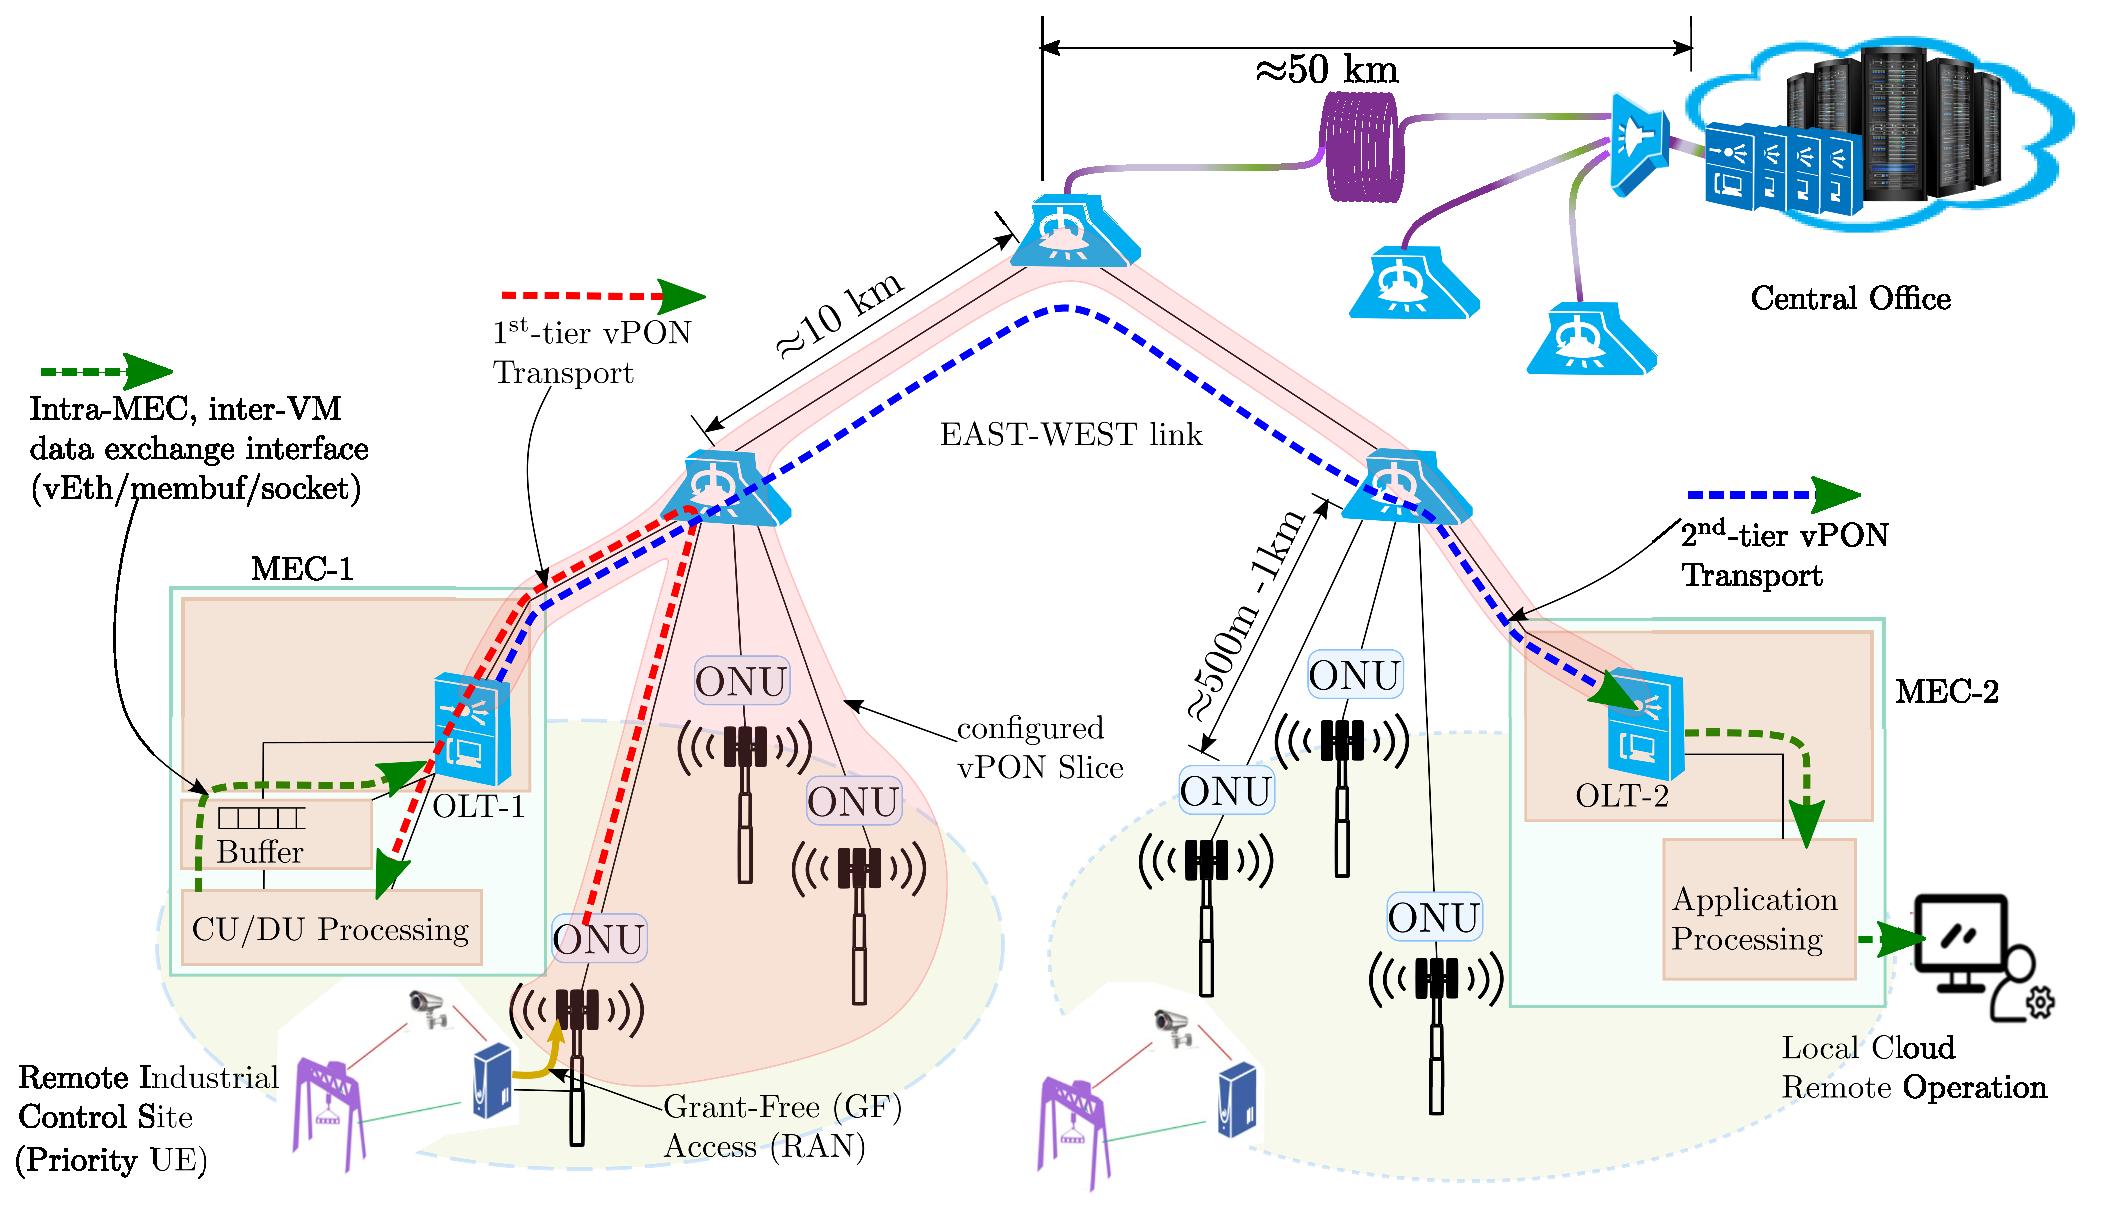
\includegraphics[clip, trim={0, 0, 0, 0}, width=\linewidth]{./Figures/SystemArc}
		\caption{System architecture for our Variable Bandwidth Fronthaul approach to cloud-RAN}
		\label{fig:SystemArc}
	\end{figure*}

	Fig. \ref{fig:SystemArc} presents the system architecture and use case. We consider a \ac{TWDM}-\ac{PON} based mobile fronthaul shared with residential users where RUs connect with CU/DU processing at \ac{CO} via two-stage splitter hierarchy. We also consider MEC nodes with limited processing capacity is deployed in the macrocell site, where the CU/DU processing can be virtualized (vCU/vDU). The transport netowrk connectivity between \ac{RU}, \ac{MEC} nodes, and \ac{CO} is enhanced with our previously proposed MESH-PON architecture \cite{MESH-PON} in order to ensure low transport latency. [write the use remote industrial use case and describe the positioning of the CU/DU and application processing elements]
	
	In this proposal, we use two cascaded vPON transport to get end-to-end application level traffic, one to transport the fronthaul data to the DU (red link) and another to transport the CU/DU processed data to the application (blue link). The first tier vPON transport (which is always an uplink) employs our proposed approach of coordinated DBA configured to incorporate the CGS resources to achieve both ultra-low fronthaul and RAN access latency. The data is processed for DU and possibly CU at the MEC-1 and to be transported to the application which is hosted at MEC-2. In this work, we propose to transport this CU/DU processed data to application at MEC-2 directly over the EAST-WEST link using our proposed second-tier vPON transport. This can be done in two alternative ways. the first possible way is to configure the vPON slice of OLT-1 (at MEC-1) to include the ONU at the MEC-2 and send the traffic to MEC-2 at the application over the next downlink period of the same vPON slice. Another alternative is by configuring the vPON slice of OLT-2 (at MEC-2) to temporarily include the ONU at MEC-1 and send the traffic to MEC-2 using the uplink of the vPON slice of OLT-2. In this limited scope of this manuscript, we consider only the first alternative option of the above two (i.e., downlink on the second tier vPON transport). However, it is also worth exploring the other alternative (i.e, uplink over the second vPON slice) as there can be possible scenarios when downlink transport in second-tier is not feasible due to lack of downlink bandwidth resources for  the OLT at MEC-1. This would then require the use of low-latency uplink transport over vPON slice-2 to send CU/DU data to the application. 
	
	\section{Proposed two-tier joint vPON scheduling method for enabling application-level ultra-low end-to-end latency} \label{sec:ProposedMethod}
	\begin{figure}[h]
		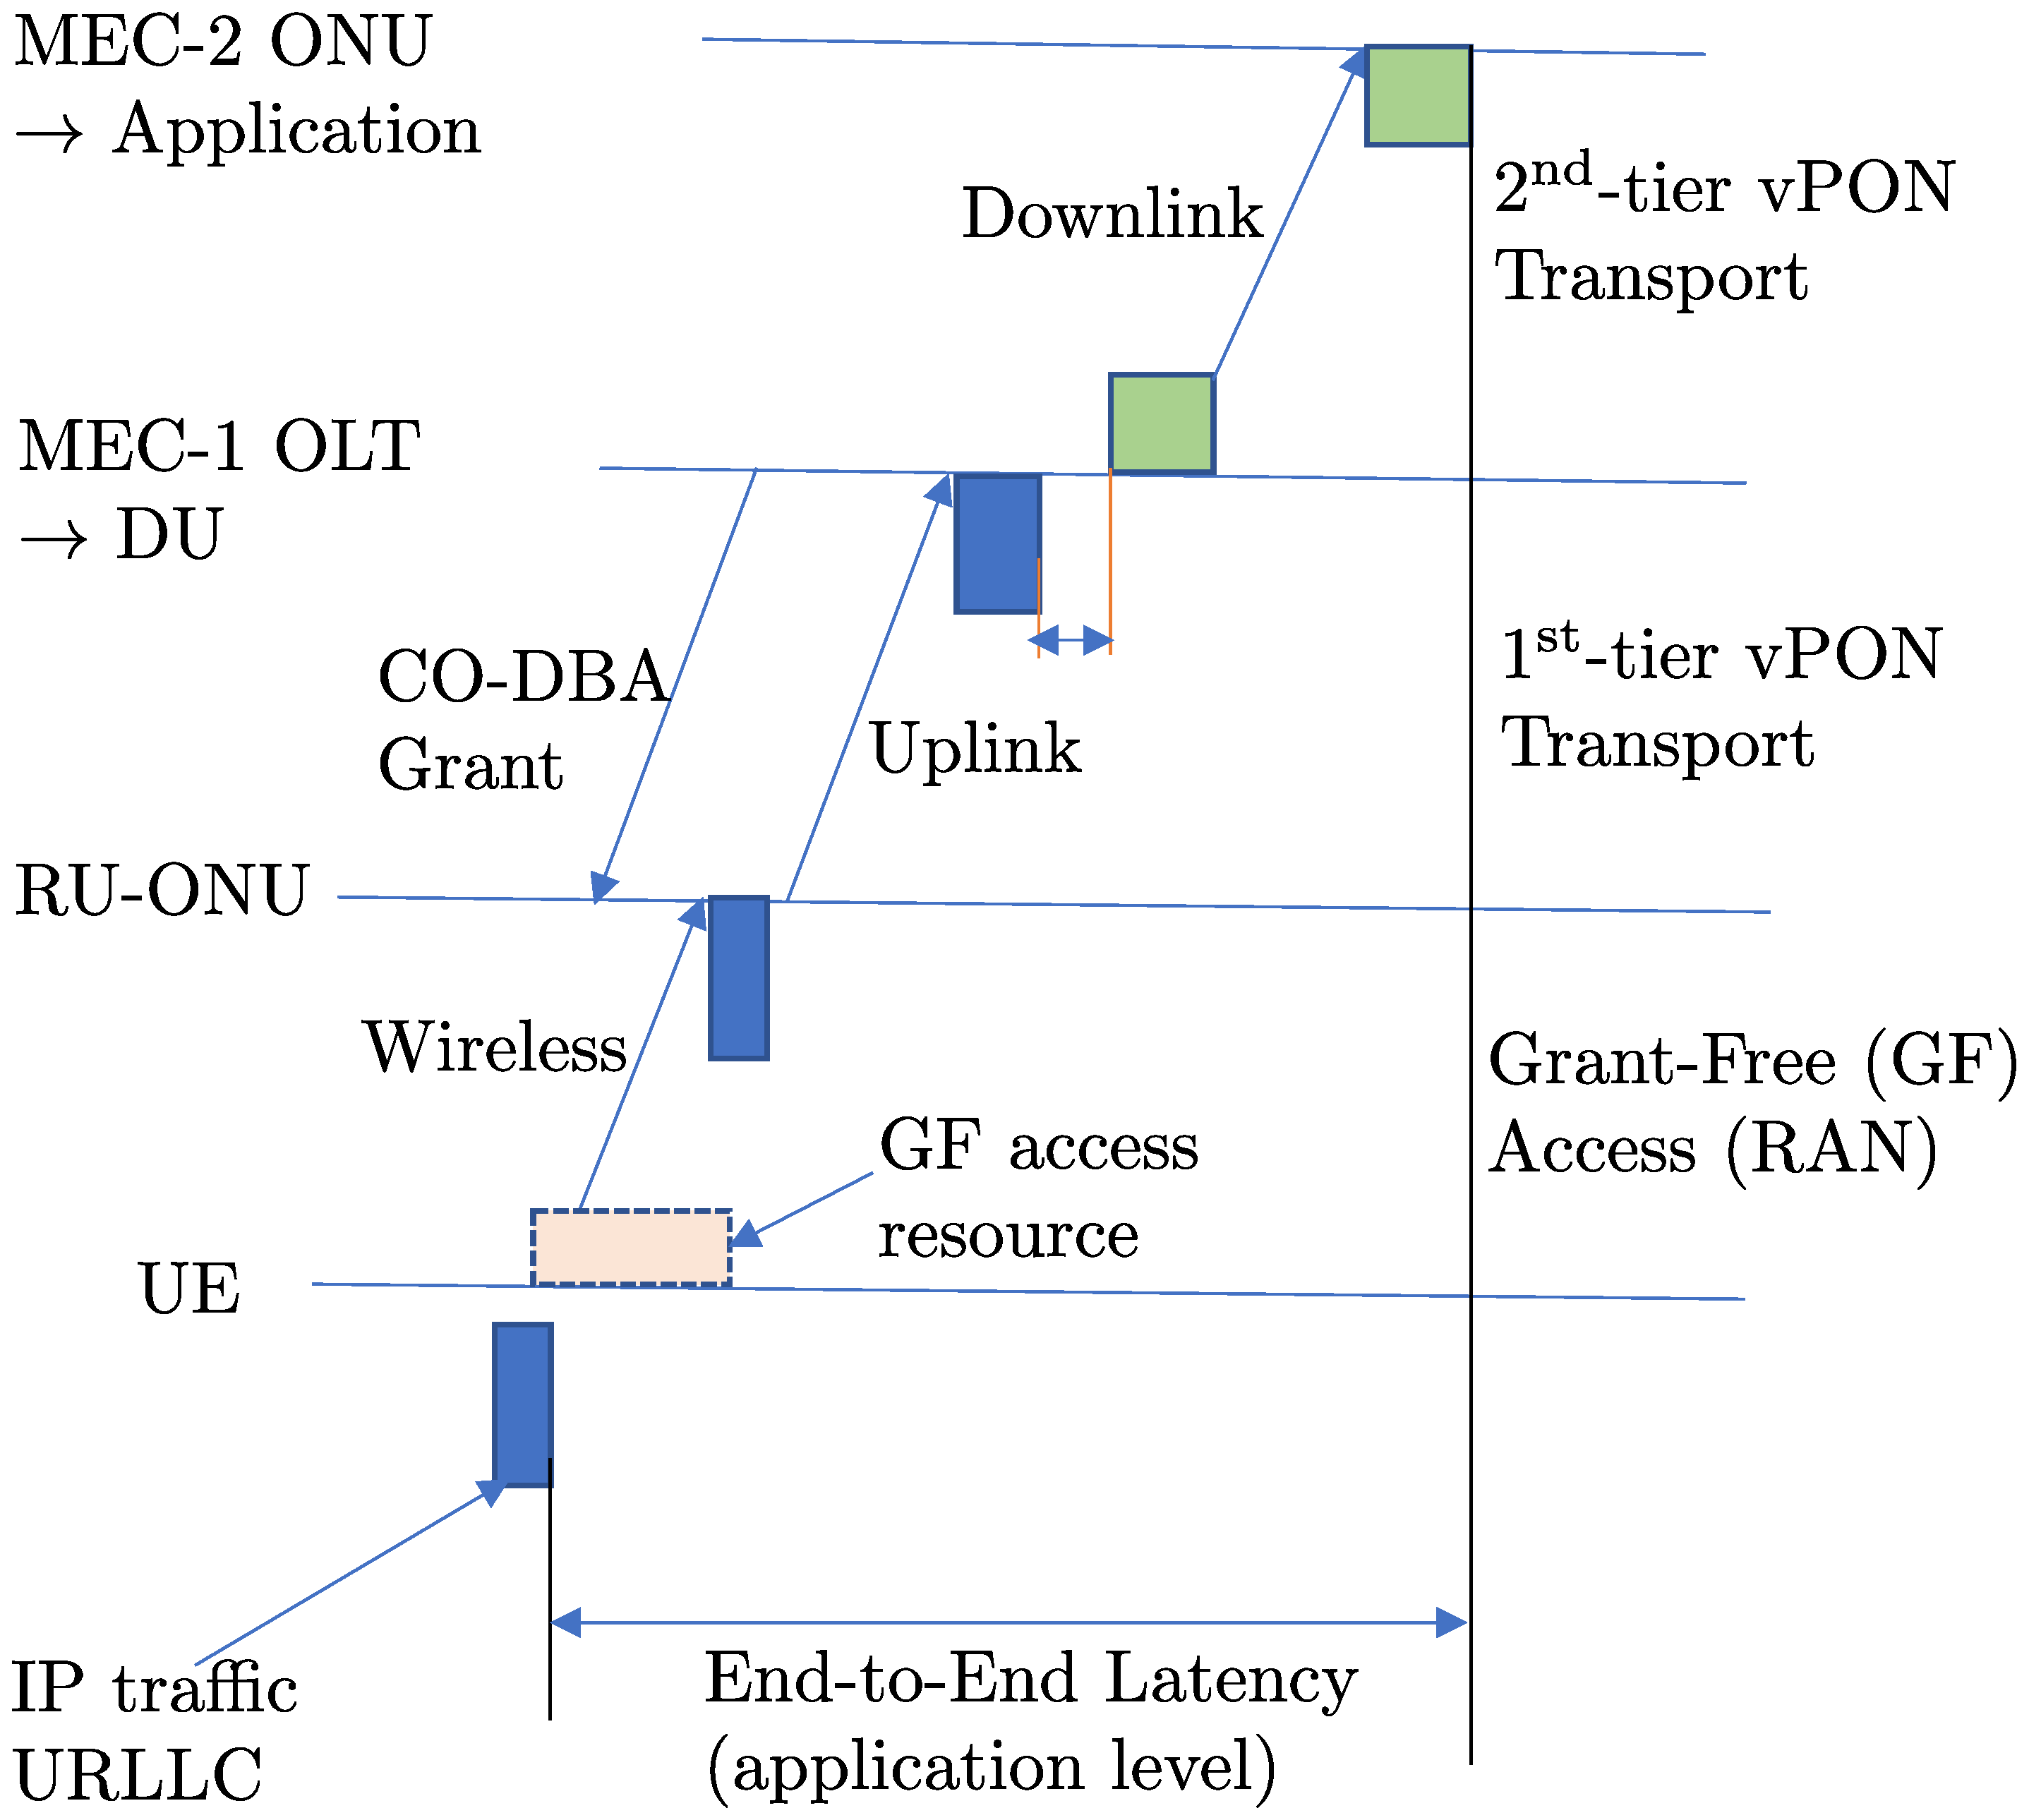
\includegraphics[clip, trim={0, 0, 0, 0}, width=\linewidth]{./Figures/DBAProtocol}
		\caption{The two-tier DBA protocol for facilitating the application-level low-latency in MESH-PON enabled MEC based Cloud-RAN}
		\label{fig:DBAProtocol}
	\end{figure}
	 The two-tier DBA protocol for facilitating the application-level low-latency is demonstrated in Fig. \ref{fig:DBAProtocol}. We consider the application level IP traffic from the UE which requires ultra-low end-to-end latency at the application level. We assume that these priority applications upon getting connected with the RU, starts sending small application level traffic of fixed size for the duration of the connection/session with the RU connected. We consider this arrival and the session time of the UE (generally referred as arrival and the holding time in terms of queuing theory) as Poisson process without the loss of any generality. As UE application has SLA for low-latency, the RRC semi-statically allocates a set of CGS resources which UE can acquire to send uplink traffic whenever it has application level packet to be transported. On the other hand, RRC passes the information of the semi-statically allocated CGS resources to the OLT to incorporate this CGS information while calculating uplink grants for CO-DBA. There are several ways to achieve this, one relatively simple and conservative approach is to include the CGS resources into account while calculating the uplink grants regardless of how many PRBs of the allocated CGS resources the UE is actually occupied depending on the current traffic. Another way is to estimate the the actual UE application and consequently estimate the percentage of the CGS resources that is occupied in the uplink and use it along with the typical mac scheduling information of calculating the grants.
	 
	 the OLT at MEC-1 dynamically configures its vPON slice to temporarily include the ONU at MEC-2 to transport the DU processed packets to the application residing at MEC-2 in the following downlink schedule. The reconfiguration of this vPON slice is facilitated prior to this at CO and the information is conveyed to the ONUs at the both MECs over the next downlink PLOAM messages as both are connected to control-channel vPON slice with CO operating over the control-channel wavelength. First, the vPON slice information is passed to ONU at MEC-1 through downlink PLOAM messages which is then passed to the OLT-1 through shared memory at the MEC-1. At the same time, the ONU at the MEC-2 receives wavelength tuning command through downlink PLOAM message to tune it's wavelength to the operating vPON wavelength of OLT-1. Upon this procedure, the OLT-1 at MEC-2 reconfigures its vPON slice and updates its DBA procedure to include ONU at MEC-2 while at the same time, the ONU at MEC-2 reconfigures its wavelength to the operating wavelength of OLT-2 to complete the reconfiguration of the vPON slice. Upon completion of the requirements of inter-MEC connectivity (for e.g., termination of the application or migration to another MEC for which the DU processed data is no longer needed to be routed to MEC-2), the ONU at MEC-2 connects back to CO-OLT control channel wavelength. This is facilitated from OLT-1 at MEC-1 via downlink PLOAM messages.
	 

    
\section{Simulation Model} \label{sec:SimulationModel}


\section{Results} \label{sec:Results}


\section{Conclusion} \label{sec:Conclusion}


\section*{Acknowledgment} \label{sec:Acknowledgment}
	Financial support from SFI 15/US-C2C/I3132, 14/IA/2527 and 13/RC/2077 \& NSF is gratefully acknowledged.

\begin{thebibliography}{99}
	\bibitem{5G-NR_Dahlman}E. Dahlman, S. Parkvall, and J. Sk\"{o}ld, ``5G NR: the next generation wireless access technology, Chapter 14: Scheduling". Elsevier, Academic Press, 2021.

	\bibitem{O-RAN-CTI} O-RAN Fronthaul Working Group 4, ``Cooperative Transport Interface Transport Control Plane Specification," O-RAN alliance, Mar. 2021.

	\bibitem{MESH-PON}S. Das, F. Slyne, and M. Ruffini. ``Optimal Slicing of Virtualised Passive Optical Networks to Support Dense Deployment of Cloud-RAN and Multi-Access Edge Computing., IEEE Network (to appear), Mar 2022, arXiv preprint arXiv:2203.11857.

	\bibitem{CPRI_Standard} Common Public Radio Interface (CPRI); Interface Specification.
	in Specification CPRI, July 2014.

\end{thebibliography}


\end{document}


%%%%%%%%%%%%%%%%%%%%%%%%%%%%%%%%%%%%%%%%%%%%%
%---------------------------------------------- End of Document -----------------------------------------------%
